\chapter{~}
I waited and waited for the sound of the house coming down, but it never came. The roar
eventually subsided, though the wind and hail did not. Eventually, the sounds of the hail quit.
The winds lessened, and the thunder started to have a little bit of distance to it again. A new
sound appeared- emergency sirens. In the background, the radio announcers were still at a
feverish pitch, describing damage, and noting that the worst of the storm had moved through
downtown. They were getting more reports from the middle of the storm from reporters to the
west, and damage reports from people where the storm had been. Power was out all over town, many
buildings had been destroyed, and many more had been damaged to various levels.

Monique was breathing very quickly and shallowly. ``Monique, are you alright?'' I asked
excitedly. She waved her hands, fighting for the air to speak. ``Yes,'' she gasped. ``Just a
little hard to get my breath with the cast on my chest.''

I wasn't sure what to do, but I started rubbing her back, making small circles on the part
that was exposed, trying to get her to calm down. It must have worked, because before long she
had regained her breath, and she turned to look at me. When our eyes met, the moment was very
awkward. I let her go, and announced that I was going to go up and take a look around. I left
her the flashlight.

I went upstairs, and looked out the back door. The sky had lightened quite a bit, and the
backyard was a mess. There were shingles, pieces of wood and siding scattered about. A bright
red piece of plastic, from some outdoor child's toy, was turning lazy circles in the pool. The
entire backyard was covered with hail- it looked like there had been a snowstorm. Over by the
garage was a stunning sight. The old oak tree had been split down the middle. One half had
remained standing, but the other half had fallen- right across the cab of my truck. The weight
of the tree had crushed the cab almost flat. I opened the back door and started to step out when
a bullhorn shouted ``STAY IN YOUR HOUSE, YOU HAVE LIVE POWER LINES DOWN!!!!'' I looked and
noticed that the tree had taken out the line to the house as it fell. I waved my thanks to the
policeman. ``DO YOU HAVE ANYONE HURT INSIDE THE HOUSE?'' he asked. ``No, we're fine!'' I yelled.
``STAY INSIDE UNTIL THE POWER COMPANY ARRIVES TO REPAIR YOUR LINES'' he said. I nodded my
assent, waved again, and shut the door.

I went through the house, checking for broken windows or any other damage as I went.
Surprisingly, I didn't see anything from the inside. I went to the front door and opened it and
looked outside. The houses across the street all looked to have varying degrees of roof damage.
There were several more large old trees down, and branches and hail covered the ground. What
caught my eye more was that many of the houses behind those seemed to be gone!

I went upstairs, again looking for damage, and not finding any. From my bedroom, which was
against the front of the house, I got a better look at the damage on the next street over, and
it looked horrible: you could see several houses with minor to moderate damage, and then a long
straight path where houses were utterly destroyed as the tornado had tracked on the ground. The
destruction path continued west for a few blocks, from what I could see.

There were already emergency vehicles everywhere. My first instinct was to go and see if I
could help in any way, but then I realized that I had been told to stay in the house, I had
power lines down in my backyard, and who knew where else. I also had a scared and mostly
helpless woman trapped in my basement. I ran back downstairs.

``How bad is it?'' Monique asked.

``It's really bad, but we got lucky. The house seems to be fine, at least from the inside.
There are power lines down, and I can't go outside right now. What's the radio saying?''

``They're telling people to stay inside if they're not hurt,'' she said. ``They're talking
about major damage to a lot of the town. They think that at least three or four tornadoes went
through.''

``Oh my God.'' I said. ``We are so lucky. Let's get you upstairs.''

I put the radio back into her lap, and wheeled her backwards to the steps. I carefully
pulled the chair up the stairs a step at a time. Considering that I was dead lifting the weight
of not only Monique, but the wheelchair and the cast, it should have been quite a struggle. For
some reason, though, it didn't seem to be difficult at all. Later, I would come to realize that
I was on an adrenaline rush, but I didn't think of it at the time. As we passed the back door,
she looked out and said. ``Oh wow- your truck.''

``Yeah, I liked that truck, too. It's nothing more than scrap, now.''

I wheeled her into the front room, and she looked out the window and gasped at the
destruction.

``We WERE lucky!''

``Yes,'' I said collapsing into a chair beside her.

``I could use a cigarette,'' she said. ``I'd get it myself, but that's not really an option
right now.''

``Yeah, I could use one, too.'' I went to go get them. When I had returned, she had used
her free hand to turn the radio back on.

``$\ldots$ Hospitals are preparing for mass casualties, but as of right now, they're still
not seeing a lot of injuries. Of course it's still too soon to say, emergency crews are
searching through neighborhoods for victims. The mayor has called in the National Guard to help
with rescue and maintaining order, as we have some serious chaos going on. If you're near the
path of destruction, authorities say you can help by hanging a red cloth out of your door if you
have anyone injured. If you don't have anyone injured, hang out a white cloth. The police want
us to tell our listeners that they will do a house to house search in the damaged areas. Hanging
a white cloth if you don't require immediate assistance will help them to reach those who need
it faster.''

I got up and retrieved an old white t shirt. I opened the front door, hung it outside, and
closed the door on it to hold it in place.

``That's a good idea.'' Monique said.

I didn't know what to say, I was still stunned.

\begin{thought}
Well, this has been quite a day, and it isn't even noon, yet! Monique was taking in the
sights outside. She was glad to see several houses across the street with white cloths hanging
from the doors. She didn't see any red ones, either. She suspected that the houses with nothing
simply were empty when the storm went through. At least she hoped so. She was concerned about
her apartment. She hoped it hadn't been hit. She'd listened to the reports on the radio from the
damage areas, and none had been from her neighborhood, at least not yet. She felt guilty, being
concerned about her apartment when people were probably hurt, maybe even dead.
She also was concerned for Quinn. He seemed to be almost in shock. As the storm raged, he'd been
a flurry of action, getting her downstairs with what seemed to be ease. Once the storm had
passed, he had comforted her, and she had truly enjoyed his embrace, even if the circumstance
was an intense one. This day would certainly be one she would not soon forget.
\end{thought}

``Quinn, are you alright? You look pale.''

``I'm OK,'' I answered. ``Or will be. I was just thinking about what could have happened to
us.''

``But it didn't.'' she said.

``I know, I know.'' I had a sudden thought. ``Monique, do you need to call anyone to see if
they're alright?''

``No,'' she answered. ``Not really. Diane is home for the summer, and my family is out of
state.'' She thought a moment and said ``Well, maybe I should call my Mom. This will probably be
on the news in Pittsburgh, and she'll worry if she sees it.''

I picked up the phone, and held it to my ear. I expected it to be dead, and I was not
surprised to find it was. I set it back down and started for the kitchen to get my cell phone.

``Line dead?'' she asked.

``Yes, hopefully the cell will work,'' I said from the kitchen.

I got the cell phone and took it back and handed it to Monique. She dialed a number, and
held it to her ear. After a few moments, she shut the phone and handed it back to me.

``The network is busy, I'll try again later.''

I sat beside her in the chair, watching the activities outside, still stunned. We sat there
for a few minutes until she broke the silence.

``So, Quinn- what are we going to do? I'd suggest hopscotch, but I don't think I'd be too
good at it right now.'' I turned to her, and she was looking at me with a slight smile. I'd
forgotten how immobilized she was, and I did not have any power to get her out of the cast
with!!!

``Shit! Shit! Shit!!!'' I yelled. ``With the power out, I can't cut you out of the
cast!!!!'' I started to panic. ``Of course, I had an AC inverter so I could do it with a car
battery, but the inverter is crushed under an oak tree, and surrounded with a live electric
line! Shit!''

``Quinn!!'' she said forcefully. ``Relax! I'm okay for the time being. We'll just wait for
the power to come back on.''

``But we don't know when that will be! This was a big storm- who knows when it will come
back on?''

Now, it was Monique who was soothing: ``Quinn, I'm okay- really. The cast isn't
uncomfortable. Let's not get crazy. We'll just deal with it. It's really not bothering me, so
let's just relax, OK?''

I calmed down a little bit, but in my mind, I was thinking of a way to get her out. She
might be OK now, but that could change. She must have sensed that I was still worried.

``Seriously, just relax. People wear casts for months at a time. I can hold out until the
power comes back on.'' \aside{And I'm not in any big hurry for it to come back on, either! She
thought to herself. I think I could wear this thing for days!}

I sat down and listened to the radio, thinking of ways to get her out without hurting her.
I could use a utility knife, but as big as the cast was, I almost certainly wouldn't get it all
cut off without slicing her. A hacksaw blade would be good, but I didn't have one. Fiberglass
wouldn't soak off in water. She was stuck. I hoped she remained as calm as she was now. I could
see it being tomorrow before power was restored, though I didn't want to tell her that.

``Please settle down, Quinn.'' She begged. ``I'm really alright. The cast is sort of like a
big hug.'' She said with a smile. ``Just keep me company, and I'll be fine.''

I couldn't help but smile back at her. ``I'm not going anywhere. And I promise that you'll
get paid overtime.'' That should make her happy.

``Ok, whatever,'' she said, waving the fingers of her casted left hand. ``I hadn't really
thought about that. Money is hardly an issue at a time like this. Let's just make this two
friends hanging out. That is, if you don't mind calling me a friend.''

The comment about the money surprised me. Maybe I WAS wrong about her.

``I don't think I mind that at all,'' I answered.

We talked for a while. We speculated on the damage from the storm. We listened to the
reports coming over the radio. There were some people injured by the storm, but there had been
no confirmed fatalities, yet. Rescue workers and utility crews were still working at a feverish
pace. The radio station could talk about nothing but the storm, switching from the newsroom to
reporters out in the areas that were hit hardest. They got reports from one reporter who was
talking about the damage the next street over.

There really wasn't much we could do about our situation. We mostly just sat and talked. I
found Monique to be a better conversationalist than I remembered. Maybe it was just the intense
situation, but I was actually enjoying being in her presence. After a while, I noticed her
trying to shift around a bit in the wheelchair.

``Are you alright?''

``Yes, but my butt is getting numb,'' she said with a smile.

``Monique, I am so sorry I can't get you out of the cast right now.''

``Relax,'' she said. ``Anyway, the cast is fine; it's just sitting in this one position
that's doing it.''

``How about if we put you in a different chair, in a different position?''

``That would be great.''

I wheeled her to a soft chair, and picked her up from the wheelchair, and set her down. She
wiggled around a bit as best she could, until she was leaning over a bit to her right, with her
left leg on the armrest, sticking straight in the air.

``There,'' she said. ``That's better.''

\begin{thought}
A lot better, she thought to herself. She was still in disbelief at the situation. She was
in this great cast, with a man she was now ready to admit she was falling for. He couldn't get
her out of the cast, and she was glad of it. One thing would make it better.
\end{thought}

``Quinn?'' Monique said. ``I've been modeling for you for a while, but there is something
that I want, but don't have.''

``What's that?'' I asked.

``You take pictures, and do great drawings of me. I'd like to have you do a drawing of me,
for me.''

That stunned me a bit. ``Monique, I'll do a sketch of you any time you want.''

``I'll pay you, of course.''

``Like hell you will,'' I replied. ``You're being so great about this mess- you're keeping
me sane. I'll do it for you for the enjoyment of it. Whenever you want it, just ask.''

``Whenever, I want, huh?'' She asked.

``Yes, whenever, no questions asked.''

``How about now?'' she smiled. ``You're in for the day, and I'm not going anywhere for a
while.''

I was really shocked by this. I started to open my mouth to ask her why she'd want a
drawing of herself in the huge cast, but before I could say the first word, she held up the
index finger of her right hand.''

``You said no questions asked.''

I had to smile. So I had. I went and got my sketch pad and pencils. I sat down across from
her, and silently started to work, still wondering why she'd want such a drawing. Oh well, I
could ask her when I was finished.

\begin{thought}
Although she hadn't known him long, this was one of her favorite ways to see Quinn. She
loved watching the intensity on his face as he worked the pencil over paper. It always made her
smile, and he always seemed to capture the smile. As he worked, she found herself lost in the
moment, only barely aware of something that was sure to cause an uncomfortable moment between
them.
\end{thought}

When I finished, I handed her the drawing.

``This is great.'' She said. ``Thank you.''

As I was about to ask her why she wanted the drawing done at this time, she said something
I'd been dreading.

``Quinn, I hate to say this, but I have to use the bathroom.''

I didn't know what to say. For purposes of modesty, I'd left her underwear on when I casted
her, and now there was no way to get the cast or the underwear off. Almost as if reading my
mind, Monique said ``I have an idea. I'll need some scissors and a towel.''

I went and got the towel, and then stopped by the casting room and got the bandage
scissors. I returned to her. She took the towel, and placed it over her lap. ``OK, now lean me
up on my left side a little.'' When I had her leaned over, she grabbed the side of her
underwear, and pulled them to her right as far as they would allow.

``OK, now cut through them as far back as you can.'' I cut through the underwear near the
back of the side strap. I thought I knew what her plan was, now. She asked me to sit her back up
straight, and when I had done so, she reached under the towel in front, and pulled the underwear
to the right from the top as far as she could, careful to not pull the towel off as she did so.

``Now, cut through them on this side,'' She said, indicating that I should cut them where
the cut would release the part holding the panties around her casted left leg. I sliced through
the material, and she pulled on it as hard as she could with her right arm. Despite her efforts,
with only one arm, and at a restricted angle, she couldn't do it.

``Can you help me with this?'' She said.

I grabbed what she'd been able to pull out, and tugged until the underwear came out.

I took her into the bathroom, and picked her up, and set her on the commode. I left, and
waited outside the door until she called me back in. She had the towel back on her lap, which I
was glad for. Despite how beautiful she was, the thought of her nude (or as close as it would
have been) would have been uncomfortable. I put her back in the wheelchair and took her back to
the living room. At that point, I had an idea of my own.

I went to my room, and found a pair of shorts that would be perfect. They were soft cotton,
with an elastic waistband. I took them back and asked Monique ``Would you rather wear something
besides a towel?''

``Yes!

It was a bit of a struggle, but we managed to get the shorts on her, which made me more
comfortable, and I think it made her feel better as well. The radio was still droning on, but it
was mostly just repeating things it had already said a dozen times or more. I walked over and
turned it off to conserve the batteries. I was trying to think of something to say when Monique
beat me to it.

``Quinn, I'm getting hungry. Are you?''

I hadn't thought about it with everything that had gone on, but I hadn't eaten anything
that morning, and I was getting hungry.

``Yes, actually I am. Want to order a pizza?'' I said with a smile.

``That would be great, but I'd hate to see the delivery time- how long do you think it
would take? A couple of days?''

``If that soon. Let me see what I've got.''

I wheeled her into the kitchen, and looked around. I had a lot of things that I could cook,
if only the stove worked. I had the makings for sandwiches, and I made us each one. I grabbed a
bag of chips, and a couple of sodas. I pushed her up to the table, angling her to it with her
right side. I sat down and we began to eat.

``It's a good thing you left one arm free or you'd have to feed me,'' she commented.

\begin{thought}
And how great would THAT be? To have both arms totally immobilized, to be totally helpless,
and having Quinn care for her every need. That would be wonderful.
\end{thought}

``Lucky for you- I have trouble feeding myself.''

``Yeah sure- you and your fumbling fingers that do those beautiful drawings.''

``That's different,'' I remarked. ``I become almost disconnected with the world when I
draw. You could march a brass band behind me when I'm sketching, and I probably wouldn't
notice.''

``However it works for you, the results speak for themselves. Your work is beautiful.''

``Thank you.''

``You're welcome.''

A few moments later, we were interrupted by a knock at the door. I went to answer it,
leaving Monique well hidden in the kitchen. I opened the door to the very welcome sight of a man
in a uniform from the power company.

``Hello, sir,'' he started. ``We're here to cut the power to the downed lines.''

My relief started to fade. ``You're not going to fix it?''

``I'm sorry sir, but I'm afraid not. Right now, we're just killing all of the downed lines
for safety purposes. We'll get the power back on as soon as we can.''

``When do you expect that to be?'' I asked him.

``It's hard to say, really- we don't know how bad things are. In the best case scenario,
sometime tomorrow. But I cannot promise that.''

My heart sank. Tomorrow. I have to get Monique out of the cast- she'll go crazy!

Not waiting for a reply, the lineman said ``We'll have that power off and the line cut back
in a few minutes. I'm sorry that's the best we can do for now.''

``OK. Thanks. Be careful.'' I said absently, as he turned to walk away.

I walked back into the kitchen, and Monique must have read the look on my face.

``Quinn, what's wrong?''

``That was the power company.''

``They're getting the power back on already?'' She said. \aside{No, not this soon. I don't
want to lose this great cast. I guess I shouldn't be greedy- I'm already on bonus time with it.
But, I really want to keep it a while longer. Maybe I just need to get the nerve to tell him.
But I don't know if I can.}

``No, they're just cutting the power. They say it will be at least tomorrow until the power
is back on.'' I looked Monique in the eye as I told her this, wanting to gauge her response if
she didn't come out and tell me. I must not be as good at reading people as I thought, because
what I saw, or thought I saw, looked almost like relief. I went on: ``We've got to figure out a
way to get you out of that cast. We could go to a motel, and take the saw, but there's an oak
tree and a squashed truck in front of the garage.''

Then I had an idea- ``Wait! We could take your car!''

``Quinn, I walked here today. My car wouldn't start.'' At that point, I remembered that she
had an umbrella when she arrived. I also remembered not seeing her car out front when we were
looking out at the damage and activity. It hadn't registered with me at the time, because of
everything else going on.

``Shit, Monique, what are we going to do? I can't leave you in that cast?!''

The next thing she said floored me.

``Why not?''

I didn't know what to say. She went on.

``Let's look at the situation. We don't have transportation, so we can't go anywhere. Even
if we did, how long would it take us to get anywhere? Right now, the roads need to be kept as
clear as possible for emergency vehicles. I'm not uncomfortable. Wearing the cast isn't so bad,
really. It's not like leaving the cast on will cause my bones to actually break. So, unless you
just hate my company, we can just wait for the power and RELAX.''

There was a time when I would certainly have hated her company. I'm still not sure that I
like it. Maybe I have read her wrong. I'm really not sure, anymore. She has said things that
almost made me believe she might actually like the casting. At the time, I just chalked it up to
greed and angling toward getting at more of the money behind this operation. But, she really
seems relaxed being in that big cast for an extended time. Maybe I was wrong, maybe she really
DOES like it, or at least have a high tolerance for it. I supposed that she could still be
angling, though. If she was, she was really good at it, and really more vile than I thought. But
I was really starting to doubt that. I really didn't know how to respond, but I managed to come
out with a feeble ``Are you sure?''

``Yes, Quinn, I'm sure. You are a hundred times more wound up over this than I am.'' She
then went back to her lunch.

After we'd finished eating, she asked if we could go sit in the parlor. I wheeled her
there, and we sat there as the afternoon sun lit the room brightly through the blinds. She
seemed to sense my emotional exhaustion, and kept the conversation going. She kept us away from
the events of the day, choosing instead to talk about a variety of subjects, including music,
which it turned out we had a lot of common ground on. We both liked classical and jazz quite a
bit. We both liked some country, but not a lot. We also both had a strong base in rock, though
she liked the recent rock trends more than I did.

Shortly, she turned the conversation to family, which was uncomfortable to me, since there
was very little I could tell her truthfully, and most everything was painful to think about. As
she talked about her family more, I reminded her to call her mother.

``You're right; I'd better call her before she worries herself to death.''

I tested the land line- still dead, as expected. I retrieved the cell phone, and she
punched the number in and held the phone to her ear. I expected that she'd not be able to get
through, but she must have gotten through, because she started speaking. I knew that she and her
family had lived in France, but I was still surprised that when she spoke to her mother, she
spoke in French. She spoke to her mother for about ten minutes, and then hung up.

``It's a good thing I called when I did,'' she said. ``The storm is national news, and she
was worried. She'd tried to call me at home, but couldn't get through. Maybe I don't have a home
any more.''

``Or maybe it's just lines down,'' I told her. ``Do you want to turn the news back on?
Maybe we might hear some reports of the damaged areas.''

``No. I think we've heard enough about the storm for one day. Some music would be nice,
though.'' Then she added with a smile: ``You know what I like.''

``Indeed, I do,'' I said as I got up and went to pick out some music. I grabbed a few CD's
and the boom box, and headed back into the parlor. I still couldn't help but enjoy the view:
Monique sitting there leaned back slightly in the wheelchair. Almost all of her tall, perfectly
shaped body was encased in hard white fiberglass. Only the right arm and leg were free, and her
beautiful face, framed nicely by her long dark hair. I wasn't sure what it was at the moment,
whether it was her beauty, the cast, or the combination of the two, but I just stood there and
stared for a moment, wishing that I could find a woman that beautiful who enjoyed casting for
the right reasons, and was not so materially oriented.

\begin{thought}
Monique wasn't sure how to react to the stare. He wasn't alarmed; she knew that from the
look on his face. She hoped he was enjoying the sight of her, though she didn't know whether he
was or not. Deep down, she truly hoped he enjoyed the sight of her in the cast, but she felt
that was asking too much. Still, she enjoyed the moment, and the fact that it gave her cause to
consider what she now knew to be a deep longing from inside her- she wanted a romantic
relationship with Quinn, and she wanted casting to play a prominent role in that relationship.
Of course, she assumed that she was asking far too much. She would have to be content with
building a friendship with him, and hoping it would develop further from there. Besides, she had
this great cast that snugly held most of her body in its delightfully unyielding grip. She knew
that this would not last forever, and that she needed to enjoy it while she had it. Quinn was
still staring at her. Maybe she should snap him out before things got uncomfortable.
\end{thought}

``Quinn, what's wrong?'' she asked.

I snapped back to reality. ``Nothing. I'm sorry; I was just lost in a thought for a
minute.''

``Penny for that thought.'' She said with a smile.

``It's not worth a penny. I'd be cheating you,'' I said as I popped in a Gershwin CD, and
pushed the play button. I sat down on the sofa next to her as the clarinet trill of ``Rhapsody
in Blue'' started. We just sat there and listened. I found myself surprised that the silence
between us was not uncomfortable, but it wasn't in the least. As we sat there, listening to the
music, I drifted off into sleep before I realized I was even tired.

\begin{thought}
Monique watched Quinn sleep. She watched the delicate rise and fall of his chest, and
listened to the gentle snoring sounds, barely audible, especially with the sounds of who knew
how many chainsaws operating around the neighborhood. This was another moment to enjoy. Again,
she tested the movement allowed her by the cast. Precious little. The cast was definitely
holding her tightly in its hard fiberglass embrace. As she thought those words, she realized
they sounded somewhat poetic, and started to compose a poem about the day so far in her head.
She wished she could write down the thoughts. She often wrote down thoughts in a notebook, and
sometimes, they took some form of prose or poetry. What was assembling itself in her head right
now would be very intense, and very private. She doubted she'd ever be able to share it with
anyone, though she wanted desperately to share the thoughts with one person- the man peacefully
sleeping on the sofa next to her. The words started to fall into place as the sun started to
fall in the West. Monique felt both highly excited and incredibly tranquil at the same time. She
snapped from her reverie as someone knocked on the door.
\end{thought}

``Quinn! Wake up!''

I snapped from sleep totally disoriented. It took a few moments to recall where I was
exactly. I looked to my right, and saw Monique, and things fell back into place in my mind.

``Quinn, someone's at the door.''

I nodded, and went to the door. I looked out, and saw it was the landlord. Although he
couldn't see Monique from where he was, if he came inside, I would have some serious explaining
to do. I opened the door.

``Hello, Harlan'' Mr. Moore said. ``I was just coming by to check on things here. It looks
like we're pretty lucky.''

``I think we were very lucky.'' I answered.

``You're alright?'' he asked.

``I'm fine. I took the basement when the siren sounded.''

``Good, it could have been a lot worse. The house came through pretty good. I don't think
you'll need to move out while the repairs are made.''

``Mr. Moore, to be honest, I haven't even seen how bad the house is damaged.'' I said.

He motioned with his hand. ``Come out and take a look.''

I went outside with him, and we turned back to look at the house. The roof had lost a lot
of shingles, but the decking underneath all looked intact. There were a couple of sections of
gutter that were dangling, and a lot of the paint had been stripped off by the wind. Other than
that, the front seemed to be undamaged, except for a red ``OK'' that had been spray painted near
the front door. That was probably done by rescue crews going house to house. They must not have
stopped to knock, since we'd hung out the cloth. We walked around to the back, and as we passed
through the gate to the backyard, he gasped. He just stared for a moment, looking at the
destroyed oak, with the largest part lying on what was left of my truck.

``Wow, that's bad. I'm sorry about your truck, but I'm glad that it didn't hit the house or
the garage!'' he said.

``Actually, so am I. The truck is a lot easier to replace than the house, or either of the
vehicles in the garage.''

``I'm sure'' he started, ``that my homeowners insurance will cover the truck.''

``Don't worry about that,'' I told him. ``I'll file it with my insurance.''

``I'll get some workers out here tomorrow or Sunday to get the tree out of the way. And
I'll get them to work on repairing the roof and gutters on Monday. I hate to run off, but I have
other tenants to check on.''

``I understand. Thanks for stopping by.''

``You're welcome,'' he said as he walked on down the block. I turned to go back inside.

``Who was that?'' Monique asked as I returned to the parlor.

``The landlord, checking on the damage.''

Again, she changed the subject away from the storm. ``Quinn, I noticed your chess set while
you were asleep. It is absolutely beautiful. Do you play?''

``I am so sorry I fell asleep on you. I didn't even know I was tired. Yes, I play.''
Actually, I loved to play, as long as the opponent was close in skill to me. I never minded
losing, but I hated playing someone whom I could beat effortlessly every time.''

She smiled and said ``I challenge you to a game, sir.''

She certainly had a way about her; I had to give her that. She had a slight flair for the
dramatic, but not excessively so.

``And I accept the challenge, ma'am. I'll set things up, you just sit where you are,'' I
answered with a smile.

``Alright, but only if you insist.''

I went to the casting room, and cleared off the casting cart. The height would be about
perfect. I set the remaining rolls of padding and fiberglass on the casting table, and wheeled
the cart out into the parlor. I placed the board on top of the cart next to the wheelchair on
her right. I then went back and got the stool, as it would be about the right height for me to
sit as we played. I had placed the board with the White pieces towards her, and she advanced a
pawn forward two spaces. ``I guess it's appropriate that I should be white, considering my
apparel,'' she said.

We played the game for almost an hour, until the sun dropped to where we had precious
little light in the room.

I thought of the candles I had stored under the kitchen sink. I asked Monique to wait a
moment, and I went and retrieved two new tapers, and small brass holders. I lit the candles, and
we continued playing by candlelight. Monique was definitely a talented player; she beat me the
first game. When I asked for a rematch, she replied ``Only if you feed me first.''

I thought for a moment, and decided to do something better than I had for lunch. I realized
that I had a perfectly functioning gas grill in the garage, and plenty of food in the kitchen.

``I think a nice steak dinner would be appropriate after such a Spartan lunch,'' I
announced.

``Exactly how do you propose to cook this steak?'' She asked. She wasn't challenging in her
question, she sounded almost playful in the way she asked it.

``Ah, if you'd simply have faith in me.'' I stepped behind her, and began pushing the
wheelchair to the kitchen. I opened the back door, and wheeled her out onto the deck. I didn't
have to worry about her being seen- the privacy fence kept the deck out of view in broad
daylight, let alone at dusk, when none of the streetlights were working.

I left Monique on the deck, and went to the garage. I got the grill, and wheeled it out and
up to the deck. I turned on the gas, and pushed the button to start the burners. I excused
myself for a moment, and went inside. I got a package with two T-bones in it. I grabbed a couple
of potatoes, and wrapped them in aluminum foil. I carried it all out to the grill. I placed the
steaks on the lower rack, and the potatoes on the upper. I closed the grill, and went back
inside, this time to retrieve cooking utensils, as well as plates and settings. I found the
small table and two chairs that had been on the deck lying against the fence several yards away.
I picked them up, and put them back on the deck.

``If you don't mind, we'll just eat out here.'' I told her.

``Sounds great to me, but it's a little chilly,'' she said.

I ran back inside, and got a blanket. I also grabbed the candles, the lighter, and our
cigarettes. As an afterthought, I stopped at the refrigerator, and grabbed a couple of beers.
Back outside, I covered her with the blanket, and lit the candles. She was very beautiful by
candlelight. I realized her beauty was affecting me. What I did not realize at the time was that
I was more comfortable in her presence than I ever was before. The rest of the world seemed a
million miles away, though it was still making its presence known mostly with the sounds of
vehicles, and the distant glow of emergency lighting in several places. I barely noticed it.

I finished cooking the steaks. As it turned out, she likes hers medium well, the same as I
do. I served up the steaks with the potatoes. I cut hers up for her, and we began to eat.

\begin{thought}
As she ate, Monique thought to herself ``I have got to tell him. I don't know if I can keep
it inside any more.'' The combination of a nice dinner outside by candlelight (by necessity, but
none the less romantic) and being with Quinn, and being casted made her feel like she was in a
dream. She thought that maybe she should pinch herself, but then realized that it would be
pretty difficult to do so, immobilized as she was. That thought made her chuckle out loud.
\end{thought}

``OK, now I'm offering a penny for YOUR thoughts'' I said.

\begin{thought}
Monique thought to herself how to word it, and decided that she couldn't. Not yet, anyway.
\end{thought}

``I was just laughing at how I'd planned to watch some TV tonight, and have a frozen
dinner,'' she said. (Not entirely a lie, she HAD planned to do that) ``This is quite a bit
different.''

``I cannot begin to say how sorry I am for everything that happened today,'' I told her.

``You have nothing to apologize for. And even if you're sorry, I'm not.''

I didn't quite know what to say to that, so I didn't say anything. I went back to eating.
After we were done, she asked if we could play the next game of Chess out there on the deck. I
cleared the table, put the dishes in the sink, and took the chessboard outside. We played two
more games, and I managed to beat her twice, but only barely. We talked awhile longer, losing
track of the time. By the time I thought to go back in and grab my watch, which was the only
timepiece in the house that was still working, it was 12:30 am. Monique's eyes had a sleepy look
to them, so I took her back into the house, and helped her into the bathroom again.

When she was done, I took her into the simulated hospital room, and hoisted her onto the
bed. I handed the controller to her, and she adjusted the bed for a few minutes until she found
a position she liked.

``Monique, I'm going to bunk down on the couch, just outside the door. That way, if you
need anything, you can just give me a yell, and I'll be close. I'm glad I had the idea to get
this bed. It's worth its weight in gold tonight.''

``Quinn,'' she asked, ``would you sit with me for a while?'' She patted the bed next to
her, and used her right arm and leg to scoot herself awkwardly to her left, making room for me.

``I sat down on the bed, and lay back, next to her. We talked for a few moments before I
drifted back off to sleep, not realizing it was happening.

\begin{thought}
Monique turned to look at Quinn. This was the second time today she'd watched him sleep.
Though the position she was lying in was slightly uncomfortable, she wasn't in agony, and she
started to drift down to sleep, remembering the words he'd said: ``I'm glad I had the
idea to get this bed.'' No mention of the idea of the bed coming from his patron. Did that mean
that he was just a good employee- thinking ahead? Or could it mean that maybe Quinn had more of
a stake in this than he let on? And why didn't he think to call his ``boss'' to let him know
things were alright, here? Considering this was her last thought as she slipped into a sleep
filled with interesting dreams.
\end{thought}

She was not alone.

\newpage
\begin{center}
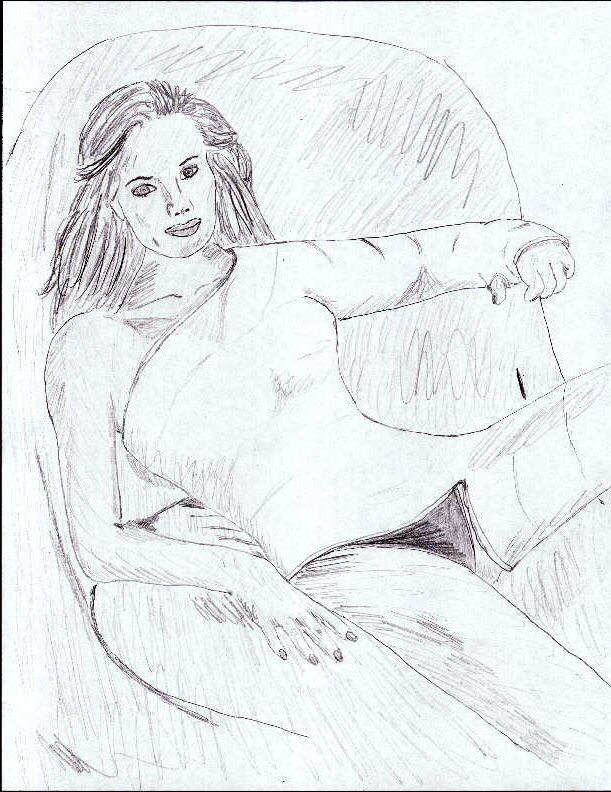
\includegraphics{images/kicks27.jpg}
\end{center}
